\documentclass[dvipdfmx,11pt]{beamer}
%\graphicspath{{fig_tab/os_presentation/20201215/}}
\usepackage{lipsum}
\usetheme{verona}
\usepackage{bxdpx-beamer}
\usepackage{pxjahyper}
\usepackage{minijs}
\usepackage{mathpazo}
\usepackage{amsmath,amssymb}
\usepackage{graphicx}
\usepackage{array}
\usepackage{tikz}
\usepackage{wrapfig}
\usepackage{float}
\usepackage{here}
\usepackage{lscape}
\usepackage{ascmac}
\renewcommand{\kanjifamilydefault}{\gtdefault}
\hypersetup{% hyperrefオプションリスト
 setpagesize=false,
 bookmarksnumbered=true,%
 bookmarksopen=true,%
 colorlinks=true,%
 linkcolor=blue,
 citecolor=blue,
 urlcolor = magenta
}
\setbeamertemplate{navigation symbols}{}

\title[Dellavigna and Linos (2022, Econometrica)]{RCTs to Scale: Comprehensive Evidence from Two Nudge Units}
\subtitle{Dellavigna and Linos (2022)}
\author{Reviewed by Reio TANJI}
\date{Apr. 12th, 2022 \\ Ohtake-Sasaki Seminar}
\institute[]{Osaka University, Graduate School of Economics}

\begin{document}

\begin{frame}\frametitle{}
\titlepage
\end{frame}

\begin{frame}{Abstract}
  \begin{itemize}
    \item A meta-analysis of Nudge interventions.
    \begin{itemize}
      \item A unique dadtaset that assembles 126 RCTs covering 23 million individuals (two of the largest Nudge Units in the U.S.).
    \end{itemize}
    \item Comparing these samples found a difference in the size of average impacts.
    \begin{itemize}
      \item Evidence from academic journals shows very large and significant impact, while that from Nudge Units are smaller.
    \end{itemize}
    \item Three dimensions accounts for these defferences.
    \begin{enumerate}
      \item Statistical power of trials
      \item Characteristics of the interventions
      \item Selective publication
    \end{enumerate}
    \item Among them, selective publication explains about 70\% of the difference in effect sizes.
  \end{itemize}
\end{frame}

\section{Introduction}
\frame{\sectionpage}

\begin{frame}{Nudge Interventions}
  \begin{itemize}
    \item Nudge 
    \begin{itemize}
      \item "\textit{choice architecture that alters perple's behavior in a predictable way without forbidding any prtions or significantly changing their economic incentives.}"
      \item have become common in the literature in fields such as economics, political science, public health, decision-making, and marketing.
    \end{itemize}
    \item Nudge Units: larger-scale applications by governments.
    \begin{itemize}
      \item Behavioral science to improve government services.
      \begin{itemize}
        \item ideas42 in the U.S. (2008)
        \item the UK's Behavioural Insights. (2010)
        \item Office of Evaluation Sciences (2015)
      \end{itemize}
      \item As of last count, there are more than 200 Nudge Units globally.
    \end{itemize}
  \end{itemize}
\end{frame}

\begin{frame}{What this paper did}
  \begin{itemize}
    \item A meta-analysis which collaborates with two major Nudge Units
    \begin{itemize}
      \item BIT North America: conducts projects with multiple U.S. local governments 
      \item OES: collaborates with multiple U.S. Federal agencies.
    \end{itemize}
    \item They conducted a total of 165 trials testing 347 nudge treatments, affecting almost 37 million participants.
    \item This paper avails 126 RCT trials, involving 241 nudges and collectively impacting over 23 million participants.
  \end{itemize}
\end{frame}

\begin{frame}{Literature of Meta-Analysis on Nudge}
  \begin{itemize}
    \item Trials to nudges: Benartzi et al. (2017) and Hummel and Maedche (2019) summarize over 100 published nudge RCTs.
    \item However, most of them have not been documented in working papers or academic publications.
    \begin{itemize}
      \item BIT and OES conducted 165 trials, but 87\% of them are not published as papers.
    \end{itemize}
    \item Evidence from their unique data set differs from a traditional meta-data analysis in:
    \begin{enumerate}
      \item The large majority of trials have not previously appeared in academic journals.
      \item No scope for selective publications.
    \end{enumerate}
  \end{itemize}
\end{frame}

\begin{frame}{Summary of Results}
  \begin{itemize}
    \item In the 26 papers in the Academic Journals sample, the average impact of nudge interventions raised take-up rate by 8.7 percentage points (33.4\%).
    \item Including all 126 trials by Nudge Units showed an unweighted impact of 1.4 percentage point (17.3\%).
    \begin{itemize}
      \item The impace is highly statistically significant, but there is large difference between two samples. 
    \end{itemize}
    \item They document three key dimensions:
    \begin{enumerate}
      \item Statistical power of trials
      \item Characteristics of the interventions
      \item Selective publication
    \end{enumerate}
    \item 1.4 percentage point impact suggests a sizeable returen on investment (with a marginal cost of typically zero or close to zero).
  \end{itemize}
\end{frame}

\begin{frame}{Contribution}
  \begin{itemize}
    \item Literature on effectiveness of nudges (Laibson, 2020; Milkman et al., 2021 etc.):
    \begin{itemize}
      \item The first comprehensive evaluation of the RCTs from Nudge Unit. 
      \item The 1.4 pp. estimate is likely a lower bound of the impact of behavioral science.
      \begin{enumerate}
        \item RCTs by Nudge Units are less likely to have characteristics associated with larger impacts such as default changes (Jachimowicz et al., 2019)
        \item The trials typically have multiple arms. 
        \item Researchers can build on the most successful results.
      \end{enumerate}
    \end{itemize}
    \item Literature on publication bias and research transparency (Simonsohn, Nelson and Simmons, 2014; Brodeur et al., 2016; Oostrom, 2021; Miguel et al., 2014; Christensen and Miguel, 2018)
    \begin{itemize}
      \item Encouraging evidence of best practices in Nudge Units.
      \item The normality assumption in meta-analyses is too restrictive (bias correction of Andrews and Kasy, 2019).
    \end{itemize}
  \end{itemize}
\end{frame}

\begin{frame}{}
  \begin{itemize}
    \item Literature on publication bias and research transparency
    \begin{itemize}
      \item Selective publication leads to the publication of resutls with large effect sizes due to luck or p-hacking.
      \item On the other hand, it may also highlight the interventions that turn out to be truly successful at inducing a behavior; "good ideas" would presumably replicate.
    \end{itemize}
    \item Literature on scaling RCT evidence (Banerjee and
    Duflo, 2009; Allcott, 2015; Bold et al., 2018; Dehejia, Pop-Eleches, and Samii, 2019; Meager, 2019; Vivalt, 2020)
    \begin{itemize}
      \item The key aspects of scaling in our setting are the ability to conduct adequately powered interventions, within the institutional constraints that are more likely to arise at scale.
    \end{itemize}
  \end{itemize}
\end{frame}

\section{Setting and Data}
\frame{\sectionpage}

\begin{frame}{Trials by Nudge Units}
  The two large Nudge Units operating in the United States:
  \begin{itemize}
    \item the Office of Evaluation Sciences (OES)
    \begin{itemize}
      \item was launched in 2015 under the Obama Administration as teh core of White House Social and Behavioral Sciences Team (SBST).
      \item OES staff work with federal agencies to scope, design, implement, and test a behavioral intervention.
    \end{itemize}
    \item the Behavioral Insights Team's North America office (BIT-NA)
    \begin{itemize}
      \item A North American office of the UK-based Behavioural Insights Team (BIT) launched in 2015.
      \item has collaborated with over 50 U.S. cities to implement behavioral experiments.
    \end{itemize}
    \item The shared goals: to use behavioral science to improve the delivery of government services through rigorous RCTs, and to build the capacity of government agencies to use RCTs.
  \end{itemize}
\end{frame}

\begin{frame}{}
  \begin{itemize}
    \item The vast majority of the trials are RCTs.
    \begin{itemize}
      \item involves a low-cost nudge using a mode of communication that does not require in-person interaction.
      \item aim to change a behavioral variable: increasing take-pu of a vaccine or reducing missed appointments.
      \item All trial protocols (including power calculations) and results are ocumented in internal registries irrespective of the results.
    \end{itemize}
    \item Taking nudge RCTs to scale in a meaningful way.
    \begin{itemize}
      \item A large sample size of trials by the governments tells us how an intervention of academic studies fares in a larger sample.
      \item tells us which academic interventions are politically, socially, and financially feasible for a government agency to implement 
    \end{itemize}
  \end{itemize}
\end{frame}

\begin{frame}{}
  \begin{figure}
    \centering
    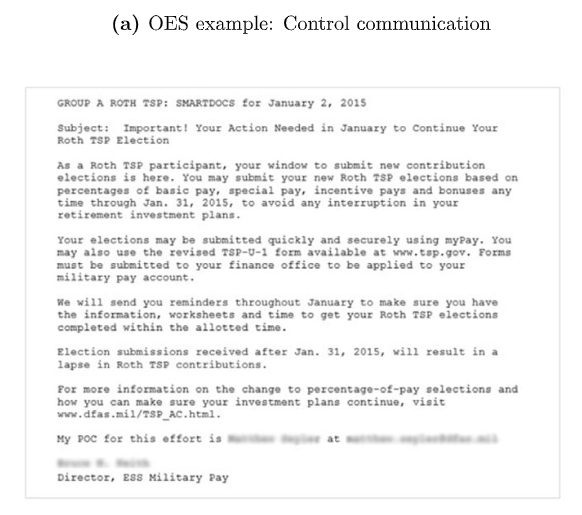
\includegraphics[scale = .55]{fig_tab/os20220412/F1a}
  \end{figure}
\end{frame}

\begin{frame}{}
  \begin{figure}
    \centering
    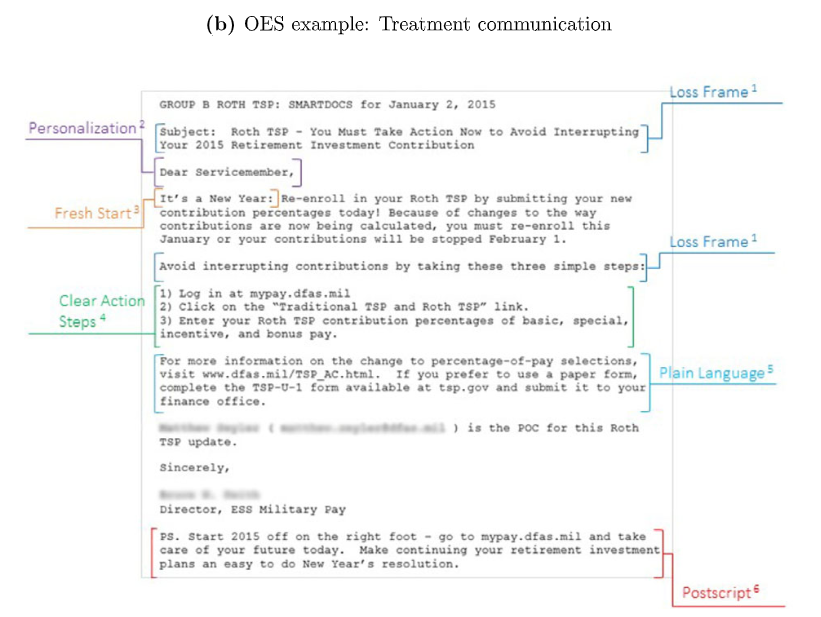
\includegraphics[scale = .5]{fig_tab/os20220412/F1b}
  \end{figure}
\end{frame}

\begin{frame}{Trials in Academic Journals}
  \begin{itemize}
    \item The authors combined the behavioral trials in Hummel and Maedche (2019) and Benartzi et al. (2017), for a total of 102 trials.
    \begin{itemize}
      \item Hummel and Maedche (2019): selected 100 papers screened out of over 2000 initial papers identified as having "nudge" or "nudging" in the title, abstract, or keyword.
      \item Benartzi et al. (2017): covers several areas and did a cost-benefit comparison of a few behavioral interventions to traditional incentive-based interventions.
    \end{itemize}
    \item The papers cover a number of disciplinary fields such as economics, public health, decision-making, and marketing.
  \end{itemize}
\end{frame}

\begin{frame}{}
  \begin{figure}
    \centering
    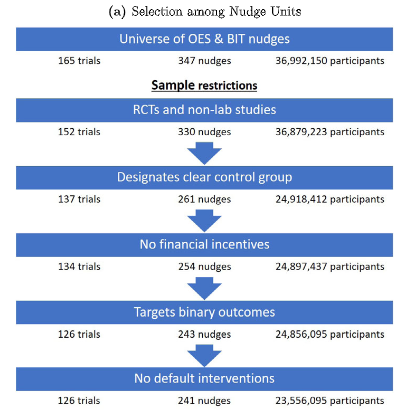
\includegraphics[scale = .5]{fig_tab/os20220412/F2a}
    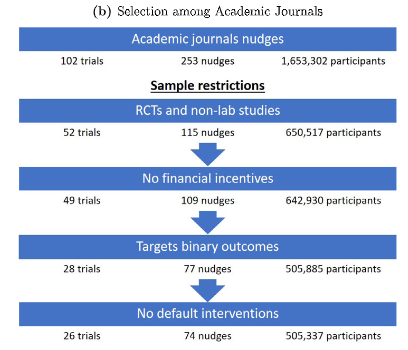
\includegraphics[scale = .5]{fig_tab/os20220412/F2b}
  \end{figure}
\end{frame}

\begin{frame}{Sample Selection}
  \begin{itemize}
    \item Trials without clear controls: horse races between two behaviorally-informed interventions.
    \item "Changing default" treatments: the rare exception among Nudge Unit interventions in the sample.
    \item The final sample consists of 126 randomized trials that include 241 nudges and involve 23.5 million participants.
    \begin{itemize}
      \item Only 16 of these trials have been written or published as academic papers.
      \item For each trial, they can observe the sample size and the take-up of the outcome variable in the control and treatment group.
    \end{itemize}
  \end{itemize}
\end{frame}

\begin{frame}{}
  \begin{figure}
    \centering
    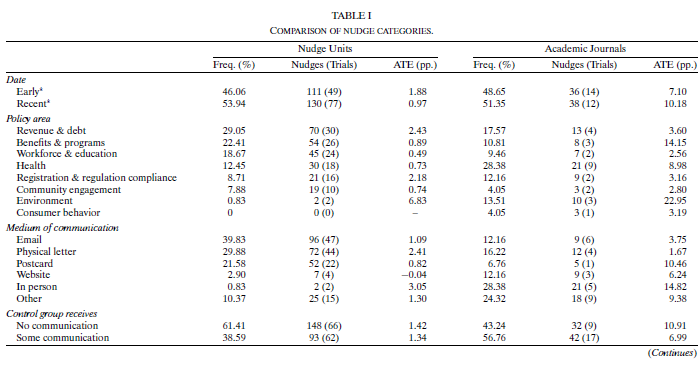
\includegraphics[scale = .5]{fig_tab/os20220412/T1}
    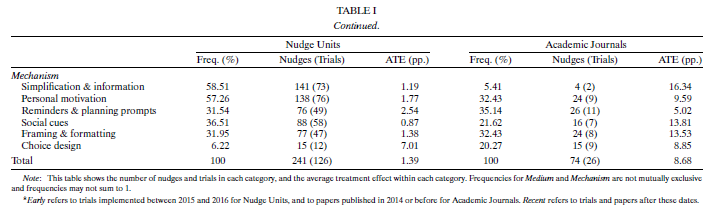
\includegraphics[scale = .5]{fig_tab/os20220412/T1b.png}
  \end{figure}
\end{frame}

\begin{frame}{Comparison of Two Samples and Author Survey}
  Categories of Nudges
  \begin{itemize}
    \item The Academic Journals sample has a larger share of trials about \textbf{health outcomes} and \textbf{environmental choices} and fewer about revenue and debt, benefits, and workforce and education.
    \item In-person interventions are common in the Academic Jounrals.
    \item Behavioral mechanisms: In the Academic Journals sample, 
    \begin{itemize}
      \item fewer cases that explicitly feature simplification and information as one of the main levers
      \item more cases that feature personal motivation and social cues, changes in framing and formatting, or choice re-design
    \end{itemize}
    \item In the Nudge Units sample, the most frequent mechanisms include: simplification of a letter or notice; drawing on personal motivation such as personalizing    the communication or using loss aversion to motivate action; using implementation intentions or planning prompts;
  \end{itemize}
\end{frame}

\begin{frame}{}
  \begin{figure}
    \centering
    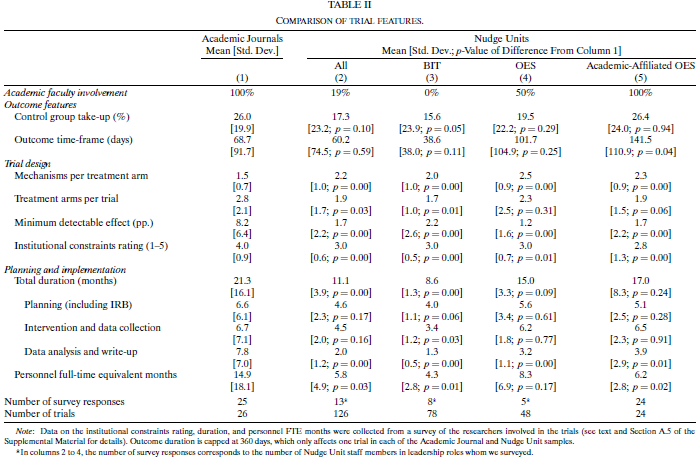
\includegraphics[scale = .66]{fig_tab/os20220412/T2}
  \end{figure}
\end{frame}

\begin{frame}{}
  Features of Trials 
  \begin{itemize}
    \item there is significant heterogeneity of the degree of academic involvement in the Nudge Units sample.
    \begin{itemize}
      \item BIT North America employs behavioral scientists and other researchers directly
      \item OES interventions are often designed in coordination with academic fellows.
    \end{itemize}
    \item the difficulty of moving a behavioral outcome: 
    \begin{itemize}
      \item Control group take-up: two samples are reasonably comparable.
      \item Time horizon of the outcome variable: The OES interventions have a longer time frame than the Academic Journals trials
    \end{itemize}
    \item Trial design
    \begin{itemize}
      \item Trials in the Academic Journals sample have fewer behavioral mechanisms per treatment arm.
      \item The average trial in the Academic Journals sample evaluates more treatment arms
      \item The typical treatment arm in the Academic Journals sample is also less statistically powered with a larger MDE
    \end{itemize}
  \end{itemize}
\end{frame}

\begin{frame}{}
  \begin{itemize}
    \item Trial design
    \begin{itemize}
      \item Short Survey of authors and of the Nudge Unit: respondents of the Academic Journal RCTs are more likely to evaluate their final interventions are close to what they initially envisioned.
    \end{itemize}
    \item Decision-making
    \begin{itemize}
      \item The average duration of the planning and intervention periods is similar for the Academic Journals sample and the OES sample (11-13 months), and somewhat shorter for the BIT sample (around 7 months).
      \item The average personnel time is higher for the Academic Journals sample than for the Nudge Units sample
      \item The data analysis and write-up period is shorter for the Nudge Unit interventions.
    \end{itemize}
    Overall, the Nudge Unit interventions are less likely to be led by academics, tend to face higher institutional constraints, and involve fewer personnel: "at scale" intervention.
  \end{itemize}
\end{frame}

\section{Impact of Nudges}
\frame{\sectionpage}

\begin{frame}{}
  \begin{figure}
    \centering
    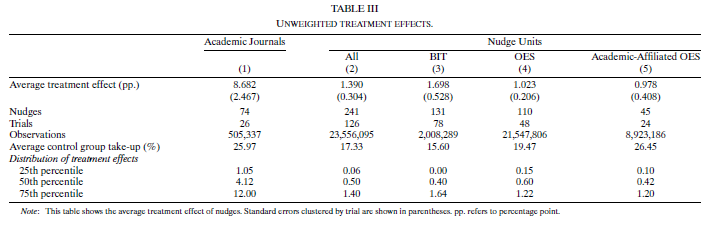
\includegraphics[scale = .6]{fig_tab/os20220412/T3}
  \end{figure}
\end{frame}

\begin{frame}{}
  \begin{figure}
    \centering
    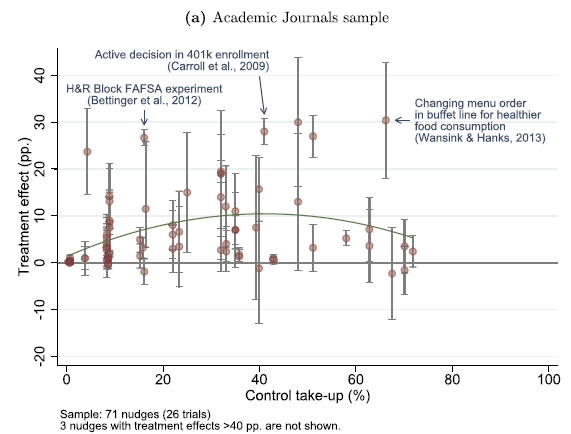
\includegraphics[scale = .6]{fig_tab/os20220412/F3a}
  \end{figure}
\end{frame}

\begin{frame}{}
  \begin{figure}
    \centering
    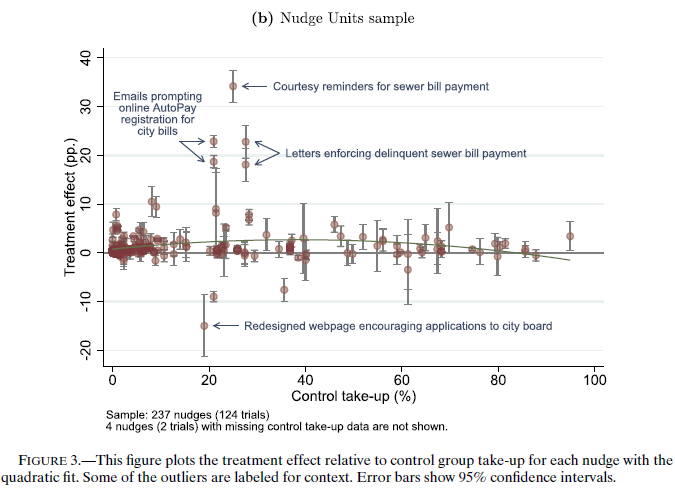
\includegraphics[scale = .6]{fig_tab/os20220412/F3b}
  \end{figure}
\end{frame}

\begin{frame}{Impact of Nudges}
  \begin{itemize}
    \item Academic Journals 
    \begin{itemize}
      \item ATE: 8.68pp. 
      \item Although there is substantial heterogeneity in the estimated impact, but nearly all the estimated effects are positive.
      \item The treatment effect is highest in settings where the control take-up rate in 20-60\%.
    \end{itemize}
    \item Nudge Units
    \begin{itemize}
      \item ATE: 1.39pp.
      \item Estimated treatment effect is sizable.
      \item Individuals effects are mostly concentrated between -2pp. and +8pp.
    \end{itemize}
    \item The statistical precision of the estimates: the confidence intervals are much tighter for the Nudge Unit studies.
  \end{itemize}
\end{frame}

\section{Nudge Units Versus Academic Journal Nudlges}
\frame{\sectionpage}

\begin{frame}{Nudge Units vs. Academic Journal Nudges}
  \begin{itemize}
    \item The authors sketch a model of decision-making around nudge experimentation. (Frankel and Kasy, forthcoming; Azevedo et al., forthcoming; Andrews and Kasy, 2019)
    \item Assumptions
    \begin{enumerate}
      \item Both academic researchers and Nudge Units design an experiment to detect an effect size $d$ with 0.80 statistical power.
      \item there is a true effect size of the nudge intervention $\beta$ distributed with a random effect.
      \item Results that are not statistically significant are published by academic researchers with some probability $\gamma < 1$, while results that are statistically significant are published with probability 1.
    \end{enumerate}
  \end{itemize}
\end{frame}

\begin{frame}{Nudge Units vs. Academic Journal Nudges}
  Under the model in the previous slide, three explanations corresponds to the followings, respectively.
  \begin{enumerate}
    \item Statistical power of trials: $d_{NU} < d_{AJ}$
    \item Characteristics of the interventions: $\beta(X_{NU}) < \beta(X_{AJ})$.
    \item Selective publication: $\gamma_{AJ} < 1$
  \end{enumerate}
\end{frame}

\begin{frame}{Experimental Design}
  \begin{itemize}
    \item the minimum detectable effect size (MDE): $d$ for 80 percent power can be computed using just the control take-up and the sample sizes in the control and treatment groups
    \begin{itemize}
      \item the Academic Journals sample has a median MDE $d_{AJ}$ of 6.30 pp. and an average MDE of 8.18 pp
      \item the Nudge Units sample has a median MDE $d_{AJ}$ of .80 pp. and an average MDE of 1.73 pp
    \end{itemize}
    \item Academic researchers expect a larger effect size than nudge practitioners.
    \begin{itemize}
      \item Researchers significantly overestimate the findings for the Nudge Units sample: different views of what is a policy-relevant or publishable effect size.
    \end{itemize}
    \item Academic Journals sample tend to try more treatment arms, which lead to lower statistical power: limited sample size is not the only the reason these differences.
  \end{itemize}
\end{frame}

\begin{frame}{}
  \begin{figure}
    \centering
    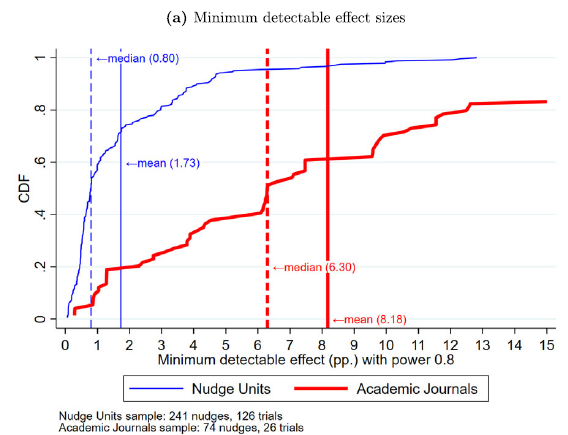
\includegraphics[scale = .6]{fig_tab/os20220412/F4a}
  \end{figure}
\end{frame}

\begin{frame}{}
  \begin{figure}
    \centering
    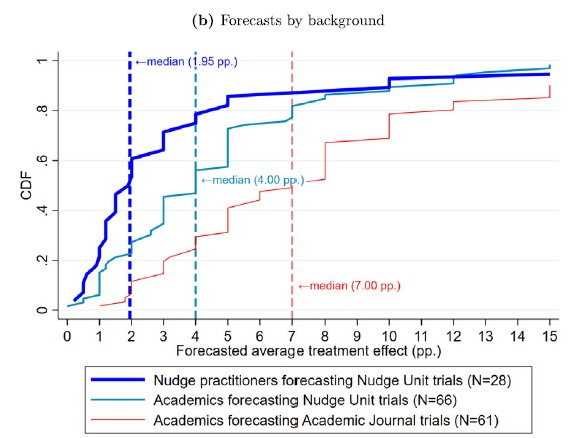
\includegraphics[scale = .6]{fig_tab/os20220412/F4b}
  \end{figure}
\end{frame}

\begin{frame}{Differences in Nudge and Trial Features}
  \begin{itemize}
    \item Academic Involvement: do not appear to explain our findings
    \begin{itemize}
      \item The average effect size for BIT interventions (1.70 pp., s.e. = 0.53) is similar to the effect size for the OES interventions desipite of the difference in some characterisitics.
      \item the 24 OES trials with explicit academic involvement, the point estimate is essentially the same as for the overall OES sample
    \end{itemize}
    \item Categories of Nudges: the average treatment effect (ATE) varies substantially across interventions.
    \begin{itemize}
      \item Prediction of nudge effect sizes: Adding controls reduce the difference in point estimate between the samples by two thirds, from 7.3 pp. to 2.4 pp..
    \end{itemize}
    \item Features of trials: features have only modest explanatory power for the effect size difference between the two samples.
  \end{itemize}
\end{frame}

\begin{frame}{}
  \begin{figure}
    \centering
    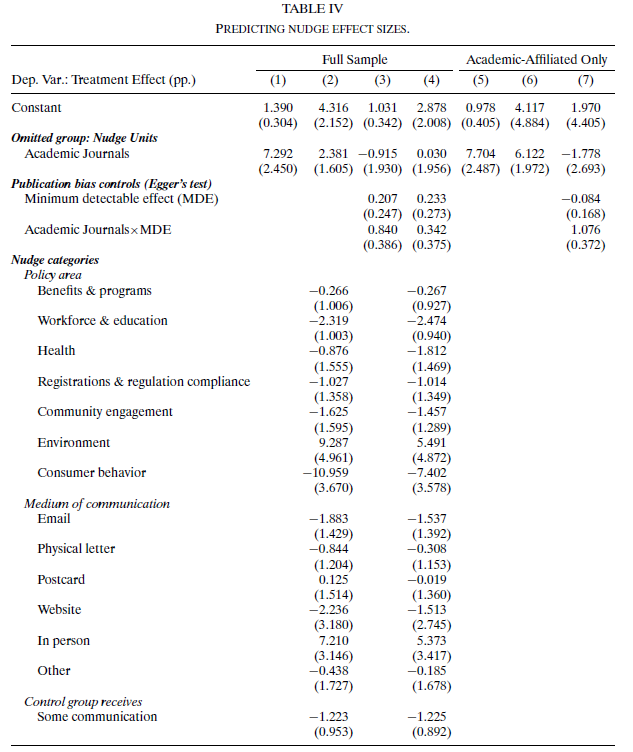
\includegraphics[scale = .4]{fig_tab/os20220412/T4a.png}
  \end{figure}
\end{frame}

\begin{frame}{}
  \begin{figure}
    \centering
    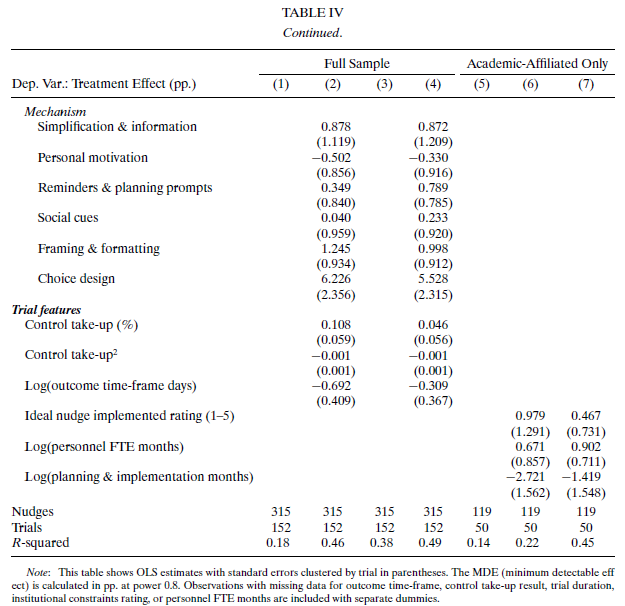
\includegraphics[scale = .5]{fig_tab/os20220412/T4b.png}
  \end{figure}
\end{frame}

\begin{frame}{Selective Publications}
  \begin{itemize}
    \item The authors does not try to distinguish the channel which leads to selective publication.
    \begin{itemize}
      \item They expect publication bias in the Academic Journals sample, but not in the Nudge Units sample.
    \end{itemize}
    \item Correlation between ATE and MDE in Academic Journal Sample:
    \begin{enumerate}
      \item The less-powered studies (studies with larger MDE) have a larger variance of the point estimates.
      \item Less-powered studies also have a larger point estimate for the nudge
    \end{enumerate}
    \item The distribution of $t$ statistics around the standard 5\% significant threshold.
    \begin{itemize}
      \item No bunching in at $t = 1.96$, but restricting treatment to those that are the most significant among every single trials suggests publication bias.
    \end{itemize}
  \end{itemize}
\end{frame}

\begin{frame}{}
  \begin{figure}
    \centering
    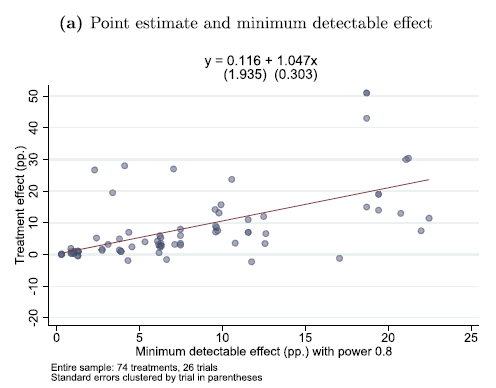
\includegraphics[scale = .45]{fig_tab/os20220412/F5a.png}
    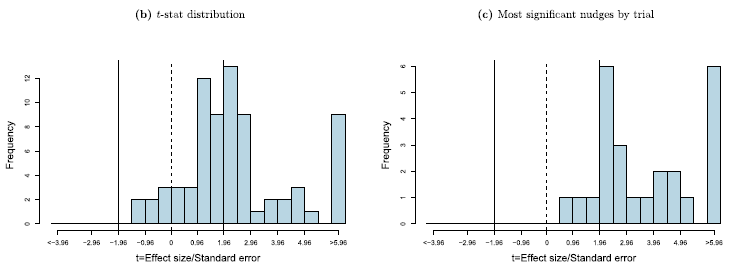
\includegraphics[scale = .5]{fig_tab/os20220412/F5bc.png}
  \end{figure}
\end{frame}

\begin{frame}{}
  \begin{figure}
    \centering
    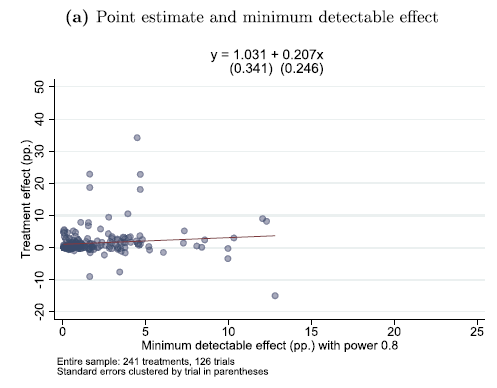
\includegraphics[scale = .45]{fig_tab/os20220412/F6a.png}
    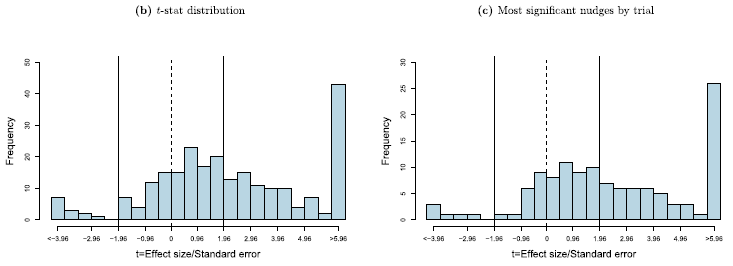
\includegraphics[scale = .5]{fig_tab/os20220412/F6bc.png}
  \end{figure}
\end{frame}

\begin{frame}{Reduced-Form Evidence of Publication Bias}
  \begin{itemize}
    \item Egger's test: controlling for statistical power (MDE) in both of two samples.
    \begin{itemize}
      \item The nudge
      effect size is strongly increasing with the MDE in the Academic Journals sample, but not in the Nudge Units sample
      \item Adding these controls can explain the entire difference in effect size.
    \end{itemize}
  \end{itemize}
\end{frame}

\begin{frame}{Meta-Analysis Model with Publication Bias Correlation}
  \begin{itemize}
    \item Andrews and Kasy (2019)'s model: A traditional random-effects meta-analysis model plus selective publication
    \begin{enumerate}
      \item Statistical power of trials: $d_{NU} < d_{AJ}$
      \item Characteristics of the interventions: $\beta_i$. The true average average effect $\bar{\beta}$ with some variance $\tau^2$, within-trial random effect model.
      \item Selective publication: $\gamma_{AJ} < 1$
    \end{enumerate}
    \item For the Academic Journal trials, selective publication accounts for about 70 percent of the larger effect size relative to the Nudge Unit trials.
  \end{itemize}
\end{frame}

\begin{frame}{}
  \begin{figure}
    \centering
    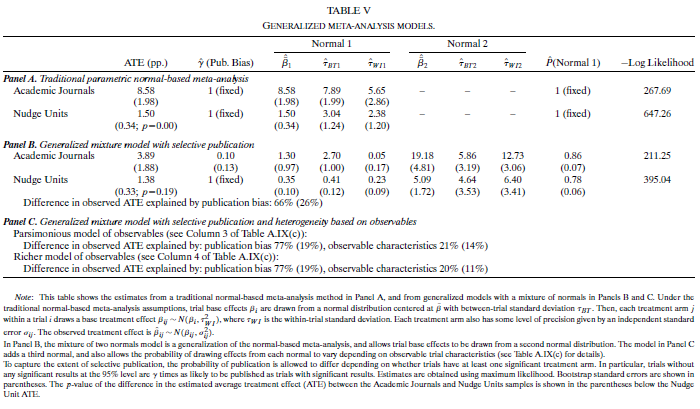
\includegraphics[scale = .6]{fig_tab/os20220412/T5.png}
  \end{figure}
\end{frame}

\begin{frame}{}
  \begin{figure}
    \centering
    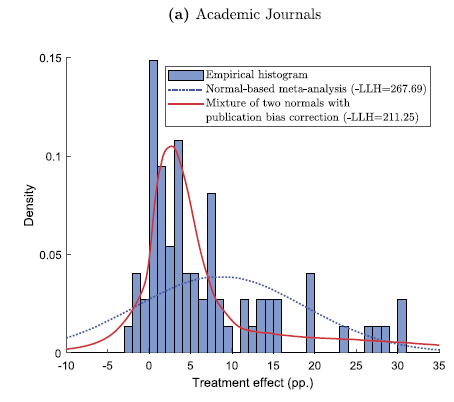
\includegraphics[scale = .5]{fig_tab/os20220412/F7a.png}
    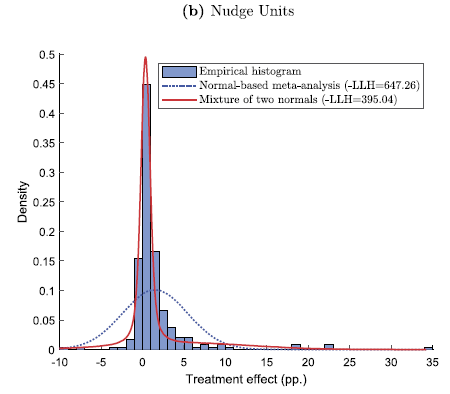
\includegraphics[scale = .5]{fig_tab/os20220412/F7b.png}
  \end{figure}
\end{frame}

\begin{frame}{Counterfactuals}
  \begin{figure}
    \centering
    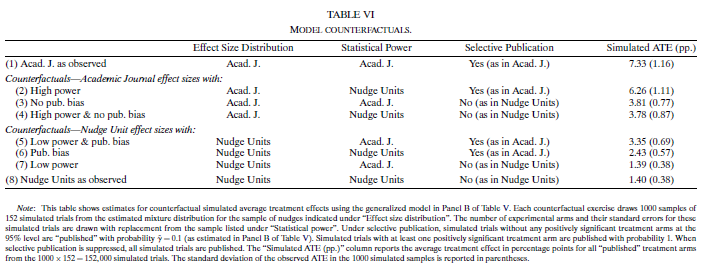
\includegraphics[scale = .65]{fig_tab/os20220412/T6.png}
  \end{figure}
  \begin{itemize}
    \item Using estimation in Table 5 to present counterfactuals.
    \item The publication bias, compounded by low statistical power explains the large effect size in the Academic Journals sample.
  \end{itemize}
\end{frame}

\section{Discussion and Conclusion}
\frame{\sectionpage}

\begin{frame}{Concluding Remarks}
  \begin{itemize}
    \item On average, nudge interventions have a meaningful and statistically significant impact on the outcome of 1.4 pp.
    \item Selective publication in the Academic Journals sample, exacerbated by low statistical power in that sample.
    \item Limitations 
    \begin{itemize}
      \item the micro-data for each trial
      \item other Nudge Units may achieve different effect sizes
      \item it would be valuable to examine determinants of which government departments decide to select into working with Nudge Units.
      \item the extent to which the results of the Nudge Unit interventions are implemented by the government units
    \end{itemize}
  \end{itemize}
\end{frame}

\end{document}
